% Created 2021-01-24 Sun 22:50
% Intended LaTeX compiler: pdflatex
\documentclass[11pt]{article}
\usepackage[utf8]{inputenc}
\usepackage[T1]{fontenc}
\usepackage{graphicx}
\usepackage{grffile}
\usepackage{longtable}
\usepackage{wrapfig}
\usepackage{rotating}
\usepackage[normalem]{ulem}
\usepackage{amsmath}
\usepackage{textcomp}
\usepackage{amssymb}
\usepackage{capt-of}
\usepackage{hyperref}
\usepackage{minted}
\hypersetup{colorlinks=true, linkcolor=black, filecolor=red, urlcolor=blue}
\usepackage[turkish]{babel}
\author{Eren Hatırnaz}
\date{20 Ekim 2019}
\title{Yazılım Gündemi - 14\\\medskip
\large 14-20 Ekim 2019}
\hypersetup{
 pdfauthor={Eren Hatırnaz},
 pdftitle={Yazılım Gündemi - 14},
 pdfkeywords={},
 pdfsubject={},
 pdfcreator={Emacs 27.1 (Org mode 9.3)},
 pdflang={Turkish}}
\begin{document}

\maketitle
\tableofcontents \clearpage\shorthandoff{=}

\begin{center}
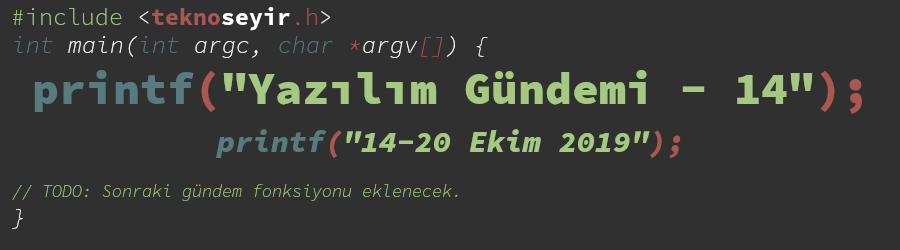
\includegraphics[width=.9\linewidth]{gorseller/yazilim-gundemi-banner.png}
\end{center}

\begin{center}
\href{../13/yazilim-gundemi-13.pdf}{< Önceki Gündem} | \textbf{14-20 Ekim 2019} | \href{../15/yazilim-gundemi-15.pdf}{Sonraki Gündem >}

\href{https://teknoseyir.com/blog/yazilim-gundemi-14-14-20-ekim-2019}{TeknoSeyir'de Oku}
\end{center}

\section{GitLab ofiste siyaset konuşmayı \href{https://www.theregister.co.uk/2019/10/16/gitlab\_employees\_gagged/}{yasakladı} ve \href{https://www.theregister.co.uk/2019/10/17/gitlab\_reverse\_ferret/}{geri aldı}}
\label{sec:orgd23c1ed}
\begin{center}
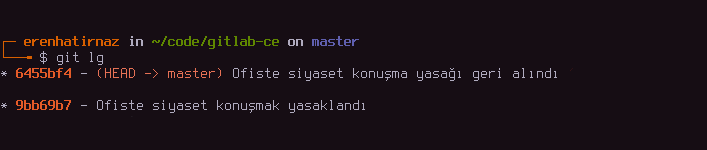
\includegraphics[width=.9\linewidth]{gorseller/gitlab-yasak.png}
\end{center}

Geçtiğimiz haftalarda bir yazılımcının ABD Göçmenlik ve Gümrük Muhafaza
kurumunu protesto etmesinden (bkz: \href{../10/yazilim-gundemi-10.pdf}{Yazılım Gündemi - 10}) ve aynı kurum ile iş
anlaşması yapmış GitHub'daki geliştiricilerin tepkilerinden (bkz: \href{../13/yazilim-gundemi-13.pdf}{Yazılım
Gündemi - 13}) bahsetmiştim. Tam da o zamanlara denk gelecek şekilde GitLab'de
"bu olaylar bizi de etkileyebilir" demiş olacak ki, CEO Sid Sijbrandij
tarafından şirketin el kitabına apar topar \href{https://gitlab.com/gitlab-com/www-gitlab-com/commit/b5a35716deb4f63299a23a40510475f5503c11c4}{bu ekleme} yapılmış. Kısaca yapılan
ekleme şu şekilde: "müşterilerimizin değerleri ile bizim değerlerimiz
uyuşmayabilir", "biz iş yerinde siyaset konuşmayız, verimlilik bizim bir
numaralı değerimizdir".

Tabii ki bu eklemeyi yaparak olası protestoların önüne geçmeyi amaçlayan şirket
yönetimi amacına ulaşamadığı gibi tam tersi bir etki de yaratıp insanların bu
konu hakkında konuşmaya başlamasına yol açtı. Her ne kadar şirketin el
kitabındaki bu değişiklik 2 hafta önce CEO tarafından \href{https://gitlab.com/gitlab-com/www-gitlab-com/merge\_requests/30656}{pull request olarak} açık
şekilde yapılmış olsa da, olay bu hafta ortaya çıktı ve tartışmalar da bu hafta
başladı. Hem şirketin kendi çalışanları hem de geliştirici camiasındaki birçok
insan reddit ve \href{https://news.ycombinator.com/item?id=21274511}{HackerNews} gibi platformlarda tepkilerini gösterdiler.

Şirketin bu yanlıştan dönmesi \href{https://www.theregister.co.uk/2019/10/17/gitlab\_reverse\_ferret/}{uzun sürmedi}. Büyüyen tartışmalar üzerine ertesi
gün şirketten yetkili başka isimler tarafından \href{https://gitlab.com/gitlab-com/www-gitlab-com/merge\_requests/32628/diffs}{sorunlu cümleler değiştirildi} ve
çalışanların iş yerinde siyaset konuşmasına yönelik yasak da kalkmış oldu.
GitLab yönetiminin bu tavırları her ne kadar doğru olmasa da şirketteki tamamen
herkese açık yapı takdir edilmesi gereken bir şey. Şirketin birçok dokümanı
herkese açık şekilde depolarında duruyor, çalışanlar de bunların
değiştirilmesinde ve geliştirilmesinde katkı verebiliyorlar. GitLab'ın bu
şekilde açık bir organizasyon yapısına olması sahip olmasını hep takdir
etmişimdir.

Bu konuda siz ne düşünüyorsunuz. Sizce GitLab yönetiminin bu şekilde
protestoların önüne geçmeye çalışması doğru mu? Yoksa çeşitli devlet
kurumlarıyla iş anlaşması yapan şirketleri protesto edenler sorunu yanlış yerde
mi arıyorlar? Yorumlar kısmında konuşalım.
\section{Python 3.8 stabil sürümü yayınlandı}
\label{sec:orgf8e49f4}
Python takımı, \href{https://www.python.org/dev/peps/pep-0569/\#release-schedule}{plan dokümanı}nda belirttikleri şekilde (hatta daha erken bir
tarihte) Python 3.8.0 final sürümünün stabil halini yayınladılar. \href{../02/yazilim-gundemi-02.pdf}{Yazılım
Gündemi - 2} yazısında Python 3.8 ile gelecek özelliklerden bazılarını
anlatmıştım. Bu yazıda onlara değinmeyeceğim fakat başka iki özelliğe birlikte
göz atalım:

\subsection{\href{https://www.python.org/dev/peps/pep-0589/}{PEP 589 - TypedDict}}
\label{sec:org3eee169}
Diğer programlama dillerinde key-value object olarak bildiğimiz yapının
Python'daki karşılığı Dictionary. Fakat Python'daki bu yapı tiplendirilmiş
şekilde kullanılamıyordu. Örnek vererek daha iyi açıklayabilirim sanırım.

Önceden bu şekilde kullanıyorduk:
\begin{minted}[breaklines=true,breakanywhere=true,frame=lines, linenos, label=Python, labelposition=topline]{python}
kisi = {'isim': 'Eren',
        'soyisim': 'Hatırnaz',
        'yas': 24}
\end{minted}

Artık bu şekilde kendi sınıfımızı oluşturup onu da Dictionary nesnesi gibi
kullanabileceğiz:
\begin{minted}[breaklines=true,breakanywhere=true,frame=lines, linenos, label=Python, labelposition=topline]{python}
from typing import TypedDict

class Kisi(TypedDict):
    isim: str
    soyisim: str
    yas: int

kisi1: Kisi = {'isim': 'Eren',
               'soyisim': 'Hatırnaz',
               'yas': 24}
\end{minted}
Yani artık tip kontrollü şekilde dictionary nesneleri kullanabileceğiz. Pek
sık Python yazmasam da ara ara benim de ihtiyacım olan bir özellikti,
gelmesine sevindim. Daha detaylı bilgi için alt başlığa eklediğim bağlantıdaki
dokümana göz atabilirsiniz.
\subsection{\texttt{final} niteleyicisi (\href{https://www.python.org/dev/peps/pep-0586/}{PEP 586 - Literal Types})}
\label{sec:orgcab0113}
Daha önce Java'da görmeye alıştığımız \texttt{final} niteleyicisi artık Python'a da
geliyor. Bilmeyenler için \texttt{final} niteleyicisi, tanımladığınız bir sınıfın,
fonksiyonun ya da değişkenin değiştirilmesi istemediğimiz durumlarda
kullandığımız bir ifade. Python da ise şu şekilde kullanabileceğiz:
\begin{minted}[breaklines=true,breakanywhere=true,frame=lines, linenos, label=Python, labelposition=topline]{python}
from typing import final

@final
class Kisi:
    @final
    def merhaba(self):
        # ..
\end{minted}
Değişkenleri ise bu şekilde değiştirilemez yapabileceğiz:
\begin{minted}[breaklines=true,breakanywhere=true,frame=lines, linenos, label=Python, labelposition=topline]{python}
ID: Final = 15
\end{minted}

Daha detaylı bilgi ve diğer değişiklikler ve yeniliklerle ilgili şeyler için
konu başlığına eklediğim bağlantıya tıklayabilirsiniz.
\section{Microsoft, .NET Framework API'lerinin .NET Core'a aktarılmasının \href{https://github.com/dotnet/announcements/issues/130}{tamamlandığını duyurdu}}
\label{sec:orga4c7369}
.NET Framework, Microsoft'un çok uzun zamandır geliştirmeye devam ettiği ve tüm
ekosistemini altında topladığı bir uygulama çatısıydı. Windows
uygulamalarından, mobil uygulamalara, oradan web uygulama ve servislerine kadar
her şey bu framework sisteminin içerisinde fakat artık Microsoft bu emektar
sistemi tozlu raflara kaldırmaya hazırlanıyor gibi. Çünkü artık .NET Framework
yalnız değil. Geçtiğimiz yıllarda gelen CEO Satya Nadella ile açık kaynak
dünyasına giriş yapan Microsoft, artık daha dışarıya açık bir yapıya sahip. Bu
değişimin ürünlerinden biri olan .NET Core projesi de .NET Framework sisteminin
yerini almaya hazırlanıyor. .NET Framework içerisindeki API'lerin de .NET Core
projesine yavaşça aktarıldığını biliyoruz. Hatta geçtiğimiz haftalarda .NET
Core 3.0 duyurulmuştu ve bu sürümle artık Windows Forms ve WPF desteğinin de
geldiğini söylemiştik (bkz: \href{../11/yazilim-gundemi-11.pdf}{Yazılım Gündemi - 11}).

Bu hafta da öğreniyoruz ki .NET Framework API'lerinin .NET Core projesine
aktarılması tamamlanmış. Yani artık .NET Framework'den hiçbir API, Core
projesine aktarılmayacak. .NET Core projesinin, \%80 civarında .NET Framework
API'si içerdiğini söylüyor Microsoft. Dolayısıyla artık .NET Framework'de
kullandığınız bazı API'ler .NET Core'da yoksa, \href{https://www.theregister.co.uk/2019/10/15/net\_framework\_port\_end/}{hiç olmayacak demektir}.

Microsoft zaten .NET'in geleceğinin Core projesi olduğunu \href{https://devblogs.microsoft.com/dotnet/net-core-is-the-future-of-net/}{bu blog yazısında}
açıklamıştı. Dolayısıyla çok da sürpriz olmadı bu gelişme. Aramızdan ayrılan
teknolojiler arasında Web Forms, WCF Server ve Windows Workflow var.
Kendilerini tozlu raflardaki yerlerine alabiliriz. .NET Framework'e destek
hemen kesilmeyecek tabii ki de fakat benim tavsiyem uygulamalarınızı artık .NET
Core altyapısına geçirmeye başlayın.
\section{Firefox geliştirici araçlarına yeni özellik eklendi: \href{https://hacks.mozilla.org/2019/10/firefoxs-new-websocket-inspector/}{WebSocket Inspector}}
\label{sec:org3e9b634}
WebSocket, sunucu ve istemci arasında kalıcı bir bağlantı kurmaya yarayan bir
teknoloji. Daha çok tarayıcı üzerinde çalışan anlık mesajlaşma uygulamalarında
kullanıyoruz. Firefox takımı da, gelen istekler üzerine yeni bir geliştirici
aracı hazırlamış ve Firefox 71 sürümünde bu aracın yer alacağını açıklamış.
Ayrıca şu an Firefox Developer Edition sürümünde bu özellik kullanılabilir
durumda. Kullanmak için F12'ye basıp DevTools penceresini açtıktan sonra,
Network sekmesine tıklayıp ve oradan da Messages sekmesine tıklamak gerekiyor.

\begin{center}
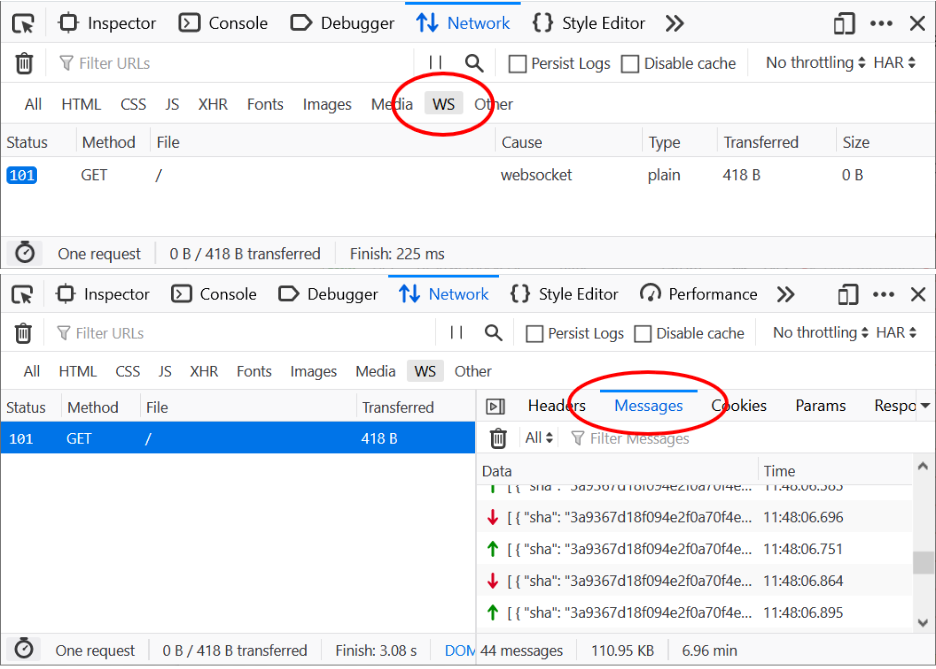
\includegraphics[height=7cm]{gorseller/websocket-inspector.png}
\end{center}

Bu WebSocket Inspector aracı ile artık sunucu ile istemci arasındaki bu veri
trafiğini izleyebilir, filtreleyebilir ve arama yapabilir hale geleceğiz. Bu
sayede de WebSocket kullanan bir uygulama geliştirirken yaşadığımız araç
sıkıntısını da çözmüş oluyor İlerleyen sürümlerde bu yeni araca yeni özellikler
de eklenecekmiş. Mozilla ve Firefox takımı yine bizim için çalışmaya devam
ediyor. <3 Mozilla <3 Firefox.
\section{Android 10 sürümünde kaldırılan bir fonksiyonellik bir \href{https://bitbucket.org/esminis/server/wiki/Home}{uygulamanın hayatına son verdi}}
\label{sec:org8296556}
Google, Android 10 sürümünde \texttt{exec()} isimli fonksiyonun uygulamaların
bulunduğu dizinde \href{https://issuetracker.google.com/issues/128554619}{çalışması engellendiği} için Servers for Android isimli
uygulamanın da geliştirilmesine son verilmiş. Uygulamanın BitBucket'daki
sayfası yayından kalmış fakat tahminime göre Android üzerinde web sunucu
çalıştırmaya yarayan bir uygulamaya benziyor. \texttt{exec()} fonksiyonu da büyük
ihtimal bir binary dosyasını çalıştırmaya yarayan bir komut (Android
geliştirici arkadaşlar yanlış biliyorsam düzeltsin beni). Bu uygulama da bu
yöntemle web sunucu için gerekli çeşitli araçları çalıştırıyormuş sanırım.
Yazıda bahsettiğine göre PHP bunlardan birisi mesela. Bu fonksiyonellik Android
10 sürümünde tamamen engellenmiş değil, eğer ilgili binary dosyaları APK
dosyasının içine paketlenmişse çalıştırılabiliyor fakat bu uygulama için bir
çözüm değil çünkü birden çok aracı ve farklı sürümlerini içermesi gerektiği
için uygulamanın boyutu 2GB'ı aşıyor ve haliyle mantıklı olmaktan da çıkıyor.
Maalesef geliştirici arkadaş uygulamayı geliştirmeyi durdurmuş ve Play
Store'dan da silmiş ama keşke BitBucket'daki kaynak kodlar dursaydı.

Maalesef geliştiricilik hayatımız boyunca böyle bir çok projemiz üzerinde
çalıştığımız platformun desteği kesmesi üzerine son bulacak. Burada Google'ın
haklılık payı var. \texttt{exec()} fonksiyonunu güvenlik sorunlarına yol açabileceği
kaygısıyla kaldırmaya hazırlanıyorlarmış.
\section{WireGuard uygulaması içerdiği \href{https://lists.zx2c4.com/pipermail/wireguard/2019-October/004596.html}{bağış bağlantısı yüzünden Play Store'dan silindi}}
\label{sec:org0ef7dd5}
Bir VPN protokolü olan WireGuard'ın Android uygulaması bu hafta bir süreliğine
Play Store'dan silindi \href{https://lists.zx2c4.com/pipermail/wireguard/2019-October/004597.html}{ve geri geldi}. Uygulamalarına kullanıcıların destek
olabilmeleri için bağış bağlantısı eklemişler ve uygulamayı Google'a inceleme
için göndermişler fakat onay beklerlerken tam tersi red edilmişler hatta
uygulama Play Store üzerinden silinmiş. Meğerse böyle bir ekleme Google'ın
"Ödeme Yönergesi"ne uygun değilmiş. Neyse ki geliştirici hızlı davranmış ve
ilgili değişikliği geri alıp tekrar incelemeye göndermiş ve uygulama kısa süre
içerisinde tekrar \href{https://play.google.com/store/apps/details?id=com.wireguard.android}{Play Store'daki yerini almış}.

Bu haber, Android geliştirici arkadaşların kulağına küpe olsun. Google'ın
sistemi dışında kullanıcılarınızdan destek almak istersiniz falan aman ha! Kapı
dışarı ederler adamı valla!
\section{Bir programlama hatası 150'den fazla \href{https://arstechnica.com/information-technology/2019/10/chemists-discover-cross-platform-python-scripts-not-so-cross-platform/}{bilimsel çalışmayı etkiledi}}
\label{sec:org01a1b2d}
Kimyasal analizde sıkça kullanılan "\href{https://www.nature.com/articles/nprot.2014.042}{Willoughby-Hoye}" isimli bir Python
betiğinin farklı işletim sistemlerinde farklı sonuçlar vermesi yüzünden 150'den
fazla bilimsel çalışma \href{https://pubs.acs.org/doi/full/10.1021/acs.orglett.9b03216}{yanlış sonuç üretmiş olabilir}.

\begin{figure}[htbp]
\centering
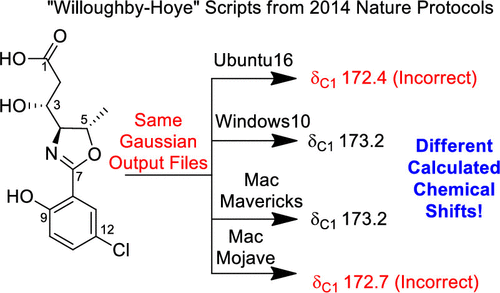
\includegraphics[width=.9\linewidth]{gorseller/programlama-hatasi-bilimi-etkiledi.png}
\caption{Betik Ubuntu 16 ve MacOS Majove sistemlerinde yanlış sonuç veriyor.}
\end{figure}

Hataya neden olan Python'daki \texttt{glob} isimli modül. Bu modül, belirli
bir şablona uygun dosya isimlerini getiren bir araç fakat bu modülün
çalışması işletim sisteminin dosyaları sıralama sistemine
bağımlıymış. Yani belirli bir şablona uygun dosya isimleri,
Ubuntu'da farklı sırayla, Windows'da farklı sırayla geliyor. Bu
habere konu olan Python betiğinde ise, \texttt{glob} fonksiyonundan gelen
dosyalar sırasıyla işleniyormuş fakat farklı sistemlerde dosyaların
da sırası değiştiği için betiğin ürettiği sonuçta buna göre
değişiyormuş. Böyle küçük bir detayı bile bulup, ortaya çıkarabilen
bilime hayranlığım sonsuz.
\section{Yaklaşan Etkinlikler}
\label{sec:org5fcb969}
\begin{longtable}{|p{8cm}|l|l|}
\hline
Etkinlik İsmi & Yer & Tarihi\\
\hline
\endfirsthead
\multicolumn{3}{l}{Önceki sayfadan devam ediyor} \\
\hline

Etkinlik İsmi & Yer & Tarihi \\

\hline
\endhead
\hline\multicolumn{3}{r}{Devamı sonraki sayfada} \\
\endfoot
\endlastfoot
\hline
\href{https://www.eventbrite.com/e/android-workshop-tickets-77583066039}{Android Workshop} & İstanbul & 22 Ekim 18:30\\
\href{https://kommunity.com/codefiction/events/codefiction-bulusuyor}{Codefiction Buluşuyor} & İstanbul & 22 Ekim 18:30\\
\href{https://kommunity.com/atolye15/events/writing-modular-scalable-and-maintainable-css}{Writing Modular, Scalable and Maintainable CSS} & İzmir & 23 Ekim 19:00\\
\href{https://www.eventbrite.com/e/yapay-zekaya-giris-semineri-tickets-75830441893}{Yapay Zekaya Giriş Semineri} & İstanbul & 24 Ekim 13:30\\
\href{https://kommunity.com/sovos-foriba-rd/events/aws-api-gateway}{AWS API Gateway} & İstanbul & 24 Ekim 17:00\\
\href{https://www.eventbrite.com/e/modern-antivirus-atlatma-teknikleri-workshop-hacknightsorg-tickets-77325327135}{Modern Antivirus Atlatma Teknikleri Workshop} & Ankara & 24 Ekim 19:00\\
\hline
\end{longtable}
\section{Diğer Haberler}
\label{sec:org69f997d}
\begin{itemize}
\item \texttt{go-yaml} projesinde DoS açığı \href{https://raesene.github.io/blog/2019/10/15/From-stackoverflow-to-CVE/}{bulundu ve giderildi}.
\item .NET Core 3.1 \href{https://devblogs.microsoft.com/dotnet/announcing-net-core-3-1-preview-1/?WT.mc\_id=dotnetcore-reddit-bramin}{Preview 1 sürümü duyuruldu}.
\item Visual Studio 2019 v16.4 \href{https://devblogs.microsoft.com/visualstudio/fall-sports-pumpkin-spice-and-visual-studio-2019-v16-4-preview-2/}{Preview 2 yayınlandı}.
\item Amazon Web Services, Rust projesine \href{https://aws.amazon.com/tr/blogs/opensource/aws-sponsorship-of-the-rust-project/}{sponsor oldu}.
\item Amazon, kendi hizmetlerindeki Oracle veritabanlarını \href{https://aws.amazon.com/tr/blogs/aws/migration-complete-amazons-consumer-business-just-turned-off-its-final-oracle-database/}{kendi çözümleri ile
değiştirdi}.
\item Microsoft'un, dağıtık uygulamalar için runtime projesi \href{https://dapr.io/}{Dapr} \href{https://github.com/dapr/dapr/releases/tag/v0.1.0}{ilk sürümü
0.1.0'ı duyurdu}.
\item Microsoft, veri görselleştirme aracı SandDance'ı \href{https://cloudblogs.microsoft.com/opensource/2019/10/10/microsoft-open-sources-sanddance-visual-data-exploration-tool/}{açık kaynak yaptı}, \href{https://github.com/Microsoft/SandDance}{GitHub
Deposu}.
\item Google Açık Kaynak Takımı, Bazel isimli build sistemlerinin ilk stabil
sürümü 1.0'ı \href{https://opensource.googleblog.com/2019/10/bazel-reaches-10-milestone.html}{genel erişilebilirlik duruma getirdi}.
\item GitHub, \href{https://itch.io/jam/game-off-2019}{Game Off} isimli oyun yarışması \href{https://github.blog/2019-10-18-get-ready-for-game-off/}{düzenliyor}.
\item Android Emulator \href{https://androidstudio.googleblog.com/2019/10/emulator-2925-canary.html}{29.2.5 Canary sürümü yayınlandı}.
\item CloudFlare deneysel olarak \href{https://blog.cloudflare.com/experiment-with-http-3-using-nginx-and-quiche/}{HTTP/3 desteği veriyor}.
\item RedHat, OpenShift 4.2 için \href{https://developers.redhat.com/blog/2019/10/16/developer-tools-openshift/}{yeni geliştirici araçlarını yayınladı}.
\item Slack, libslack isimli C++ kütüphanesini \href{https://slack.engineering/client-consistency-at-slack-beyond-libslack-c9cfbe778fb7}{geliştirmeyi durdurduğunu açıkladı}.
\item EmacsConf içeriği \href{https://emacsconf.org/2019/schedule}{belli oldu}.
\item Go programlama dilinin 1.13.3 ve 1.12.12 \href{https://groups.google.com/forum/\#!topic/golang-announce/R3XK-Wf-Mtk}{sürümleri yayınlandı}.
\item D programlama dilinin geleceği hakkında \href{https://dlang.org/blog/2019/10/15/my-vision-of-ds-future/}{bir blog yazısı yayınlandı}.
\item Swift programlama dilinin yeni diagnostic mimarisi \href{https://swift.org/blog/new-diagnostic-arch-overview/}{ile ilgili yazı
yayınlandı}.
\item Vue-cli, \href{https://app.releasly.co/releases/vuejs/vue-cli/4\_0\_0}{v4.0.0 sürümü yayınlandı}.
\item RustUp, \href{https://blog.rust-lang.org/2019/10/15/Rustup-1.20.0.html}{1.20.0 sürümü duyuruldu}.
\item Go ile yazılmış client-driven REST-API sunucusu \href{https://github.com/dunglas/vulcain}{vulcain}, ilk sürümü \href{https://github.com/dunglas/vulcain/releases/tag/v0.1.0}{0.1.0'ı
yayınladı}.
\item TinyGo \href{https://github.com/tinygo-org/tinygo/releases/tag/v0.9.0}{0.9.0 sürümü çıktı}.
\item Birden çok geliştirici aracını bir arada barındıran \href{https://github.com/reugn/dev-tools}{reugn/dev-tools}
uygulamasını \href{https://github.com/reugn/dev-tools/releases/tag/v0.2.0}{0.2.0 sürümü çıktı}.
\item uvw (C++ için \href{https://github.com/libuv/libuv}{libuv}) \href{https://github.com/skypjack/uvw/releases/tag/v2.2.0\_libuv-v1.33}{2.2.0 sürümü çıktı}.
\item watt \href{https://github.com/dtolnay/watt/releases/tag/0.1.0}{0.1.0 sürümü çıktı}.
\item fancy-regex kütüphanesinin \href{https://github.com/fancy-regex/fancy-regex/releases/tag/0.2.0}{0.2.0 sürümü çıktı}.
\end{itemize}
\section{Lisans}
\label{sec:orgef114c3}
\begin{center}
\begin{center}

\includegraphics[height=1.5cm]{../../../img/CC_BY-NC-SA_4.0.png}
\end{center}

\href{yazilim-gundemi-14.pdf}{Yazılım Gündemi - 14} yazısı \href{https://erenhatirnaz.github.io}{Eren Hatırnaz} tarafından \href{http://creativecommons.org/licenses/by-nc-sa/4.0/}{Creative Commons
Atıf-GayriTicari-AynıLisanslaPaylaş 4.0 Uluslararası Lisansı} (CC BY-NC-SA 4.0)
ile lisanslanmıştır.
\end{center}
\end{document}
